\chapter{Evaluation}

\section{Continuation Benchmarks}
These are benchmarks made by project Loom themselves using the JMH.
The benchmark contains five different classes:
\begin{itemize}
  \item Freeze
  \item Thaw
  \item FreezeAndThaw
  \item OneShot
  \item Oscillation
\end{itemize}

All classes use the same settings:
\begin{lstlisting}[language=custom-java]
    @BenchmarkMode(Mode.AverageTime)
    @OutputTimeUnit(TimeUnit.NANOSECONDS)
    @State(Scope.Thread)
    @Warmup(iterations = 5, time = 1, timeUnit = TimeUnit.SECONDS)
    @Measurement(iterations = 5, time = 1, timeUnit = TimeUnit.SECONDS)
    @Fork(1)
\end{lstlisting}
They measure the average time and return the results in nanoseconds. They run five warmup iterations before measuring. Each measurement is ran five times. The state is the default state. Forking is enabled.
\\
\\
Each class contains at least one function which is benchmarked multiple times using different parameters.
All classes except for the Oscillation class use the same two parameters. Those parameters are called paramCount and stackDepth:
\begin{lstlisting}[language=custom-java]
    @Param({"1", "2", "3"})
    public int paramCount;
    
    @Param({"5", "10", "20", "100"})
    public int stackDepth;
\end{lstlisting}
Measurement series are run for every combination of those two parameters. Resulting in 12 different measurements.
The parameters of the Oscillation class class are sligthly different:
\begin{lstlisting}[language=custom-java]
    @Param({"2", "3", "4"})
    public int minDepth;
    
    @Param({"5", "6", "7", "8"})
    public int maxDepth;
    
    @Param({"10", "100", "1000"})
    public int repeat;
\end{lstlisting}
This results in 36 runs for the Oscillation class.
\\
\\
All classes use the same core task to benchmark. It is a simple recursive function. For example, if the stackDepth is 10, the function will call itself 10 times. Depending on the paramCount and which class is being benchmarked, the recursive function will then perform certain actions at a certain stackDepth.
\\
\\
Errors of the following results can be found in the annex.
\subsection{Freeze}
The Freeze benchmark optionally yields at a certain depth. It only measures yielding. An increase in the parameter count was expected to increase the time it takes to freeze since there are more frames to copy. This behavior can only be observed at a stack depth of 100. Measurement inaccuracies might be to blame for that. An increase in stack depth consistently increases the time it takes to finish the task, as expected.

\begin{figure}[H]
  \centering
  \begin{subfigure}[b]{1.0\textwidth}
    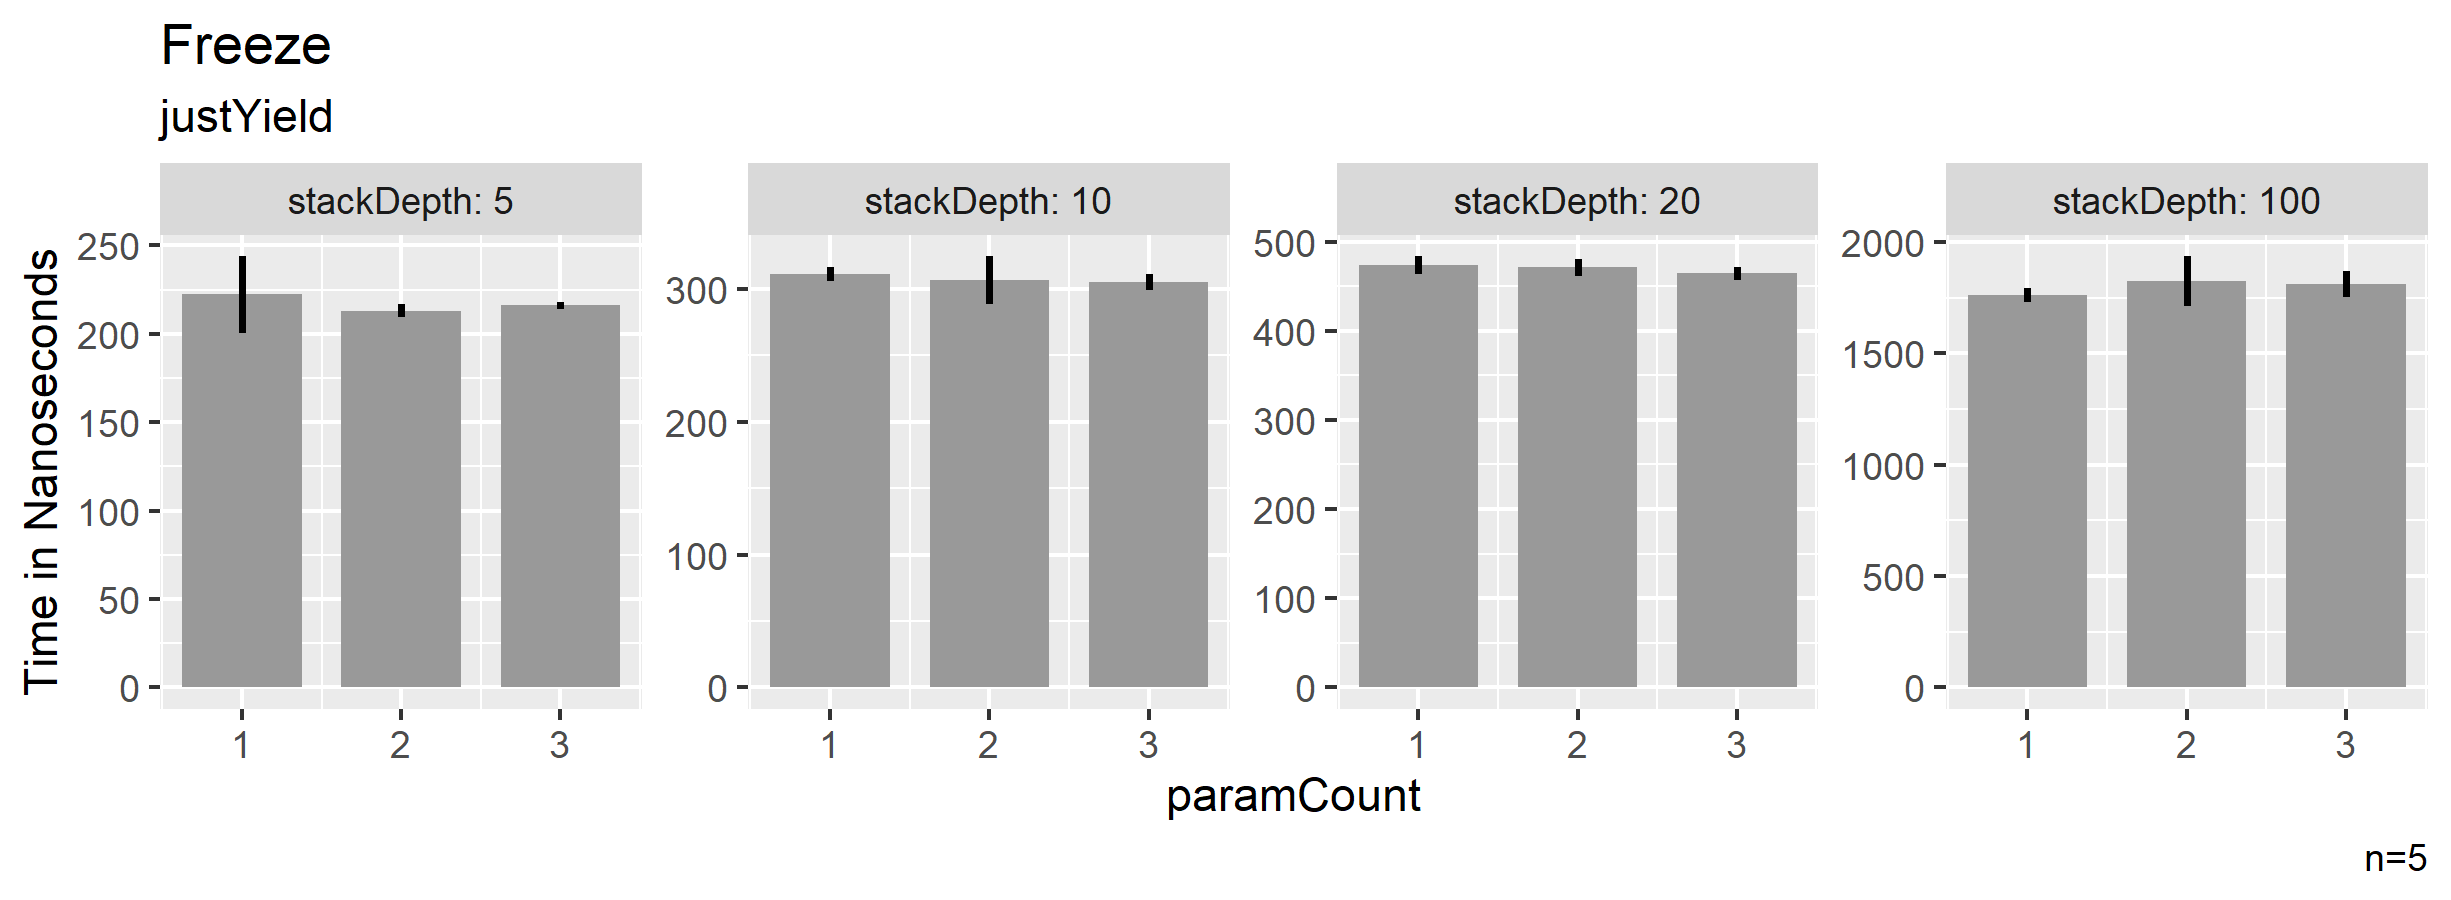
\includegraphics[width=1.0\linewidth]{img/jmh/Freeze.png}
  \end{subfigure}
  \caption{Freeze}
\end{figure}


\subsection{Thaw}
Similar to how the Freeze benchmark only measures yielding, the Thaw benchmark only measures the reverse, which is continuing. The expectations here were the same as before: Both an increase in parameter count and an increase in stack depth should increase the time. This time around only at a stack depth of 5 the results were different from the expectations.

\begin{figure}[H]
  \centering
  \begin{subfigure}[b]{1.0\textwidth}
    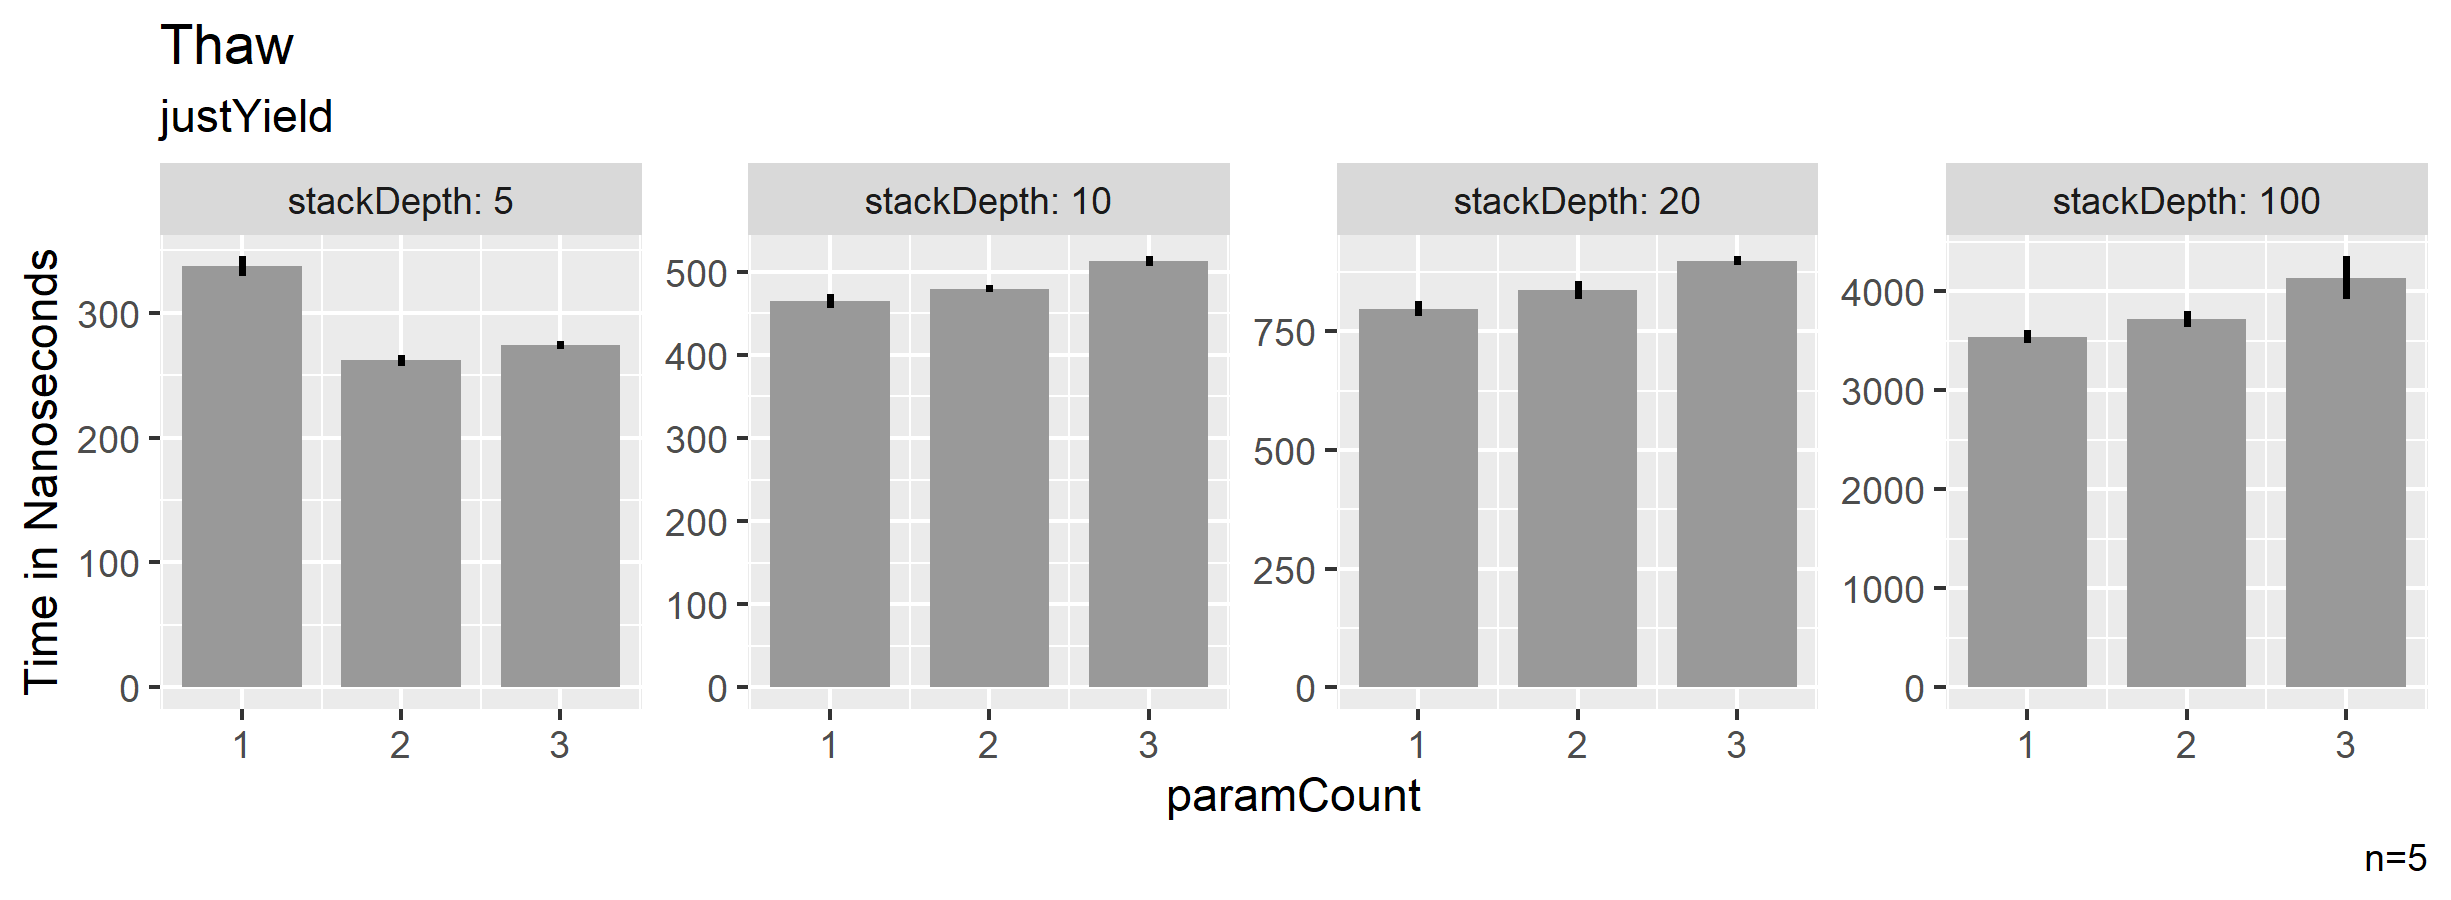
\includegraphics[width=1.0\linewidth]{img/jmh/Thaw.png}
  \end{subfigure}
  \caption{Thaw}
\end{figure}

\subsection{FreezeAndThaw}
As the name implies FreezeAndThaw measures both freezing and thawing. It runs two different methods: baseline and yieldAndContinue. The difference between those two is, that the continuation of the baseline method doesn't yield at the limit. Which means it doesn't yield at all. It just completes the task. So one can compare the baseline and the yieldAndContinue run to see how strongly freezing and thawing affected the time to finish the task. As one can see in the figure below, the impact of yielding and continuing is big. Without it, the task is completed up to 10 times faster.

\begin{figure}[H]
  \centering
  \begin{subfigure}[b]{1.0\textwidth}
    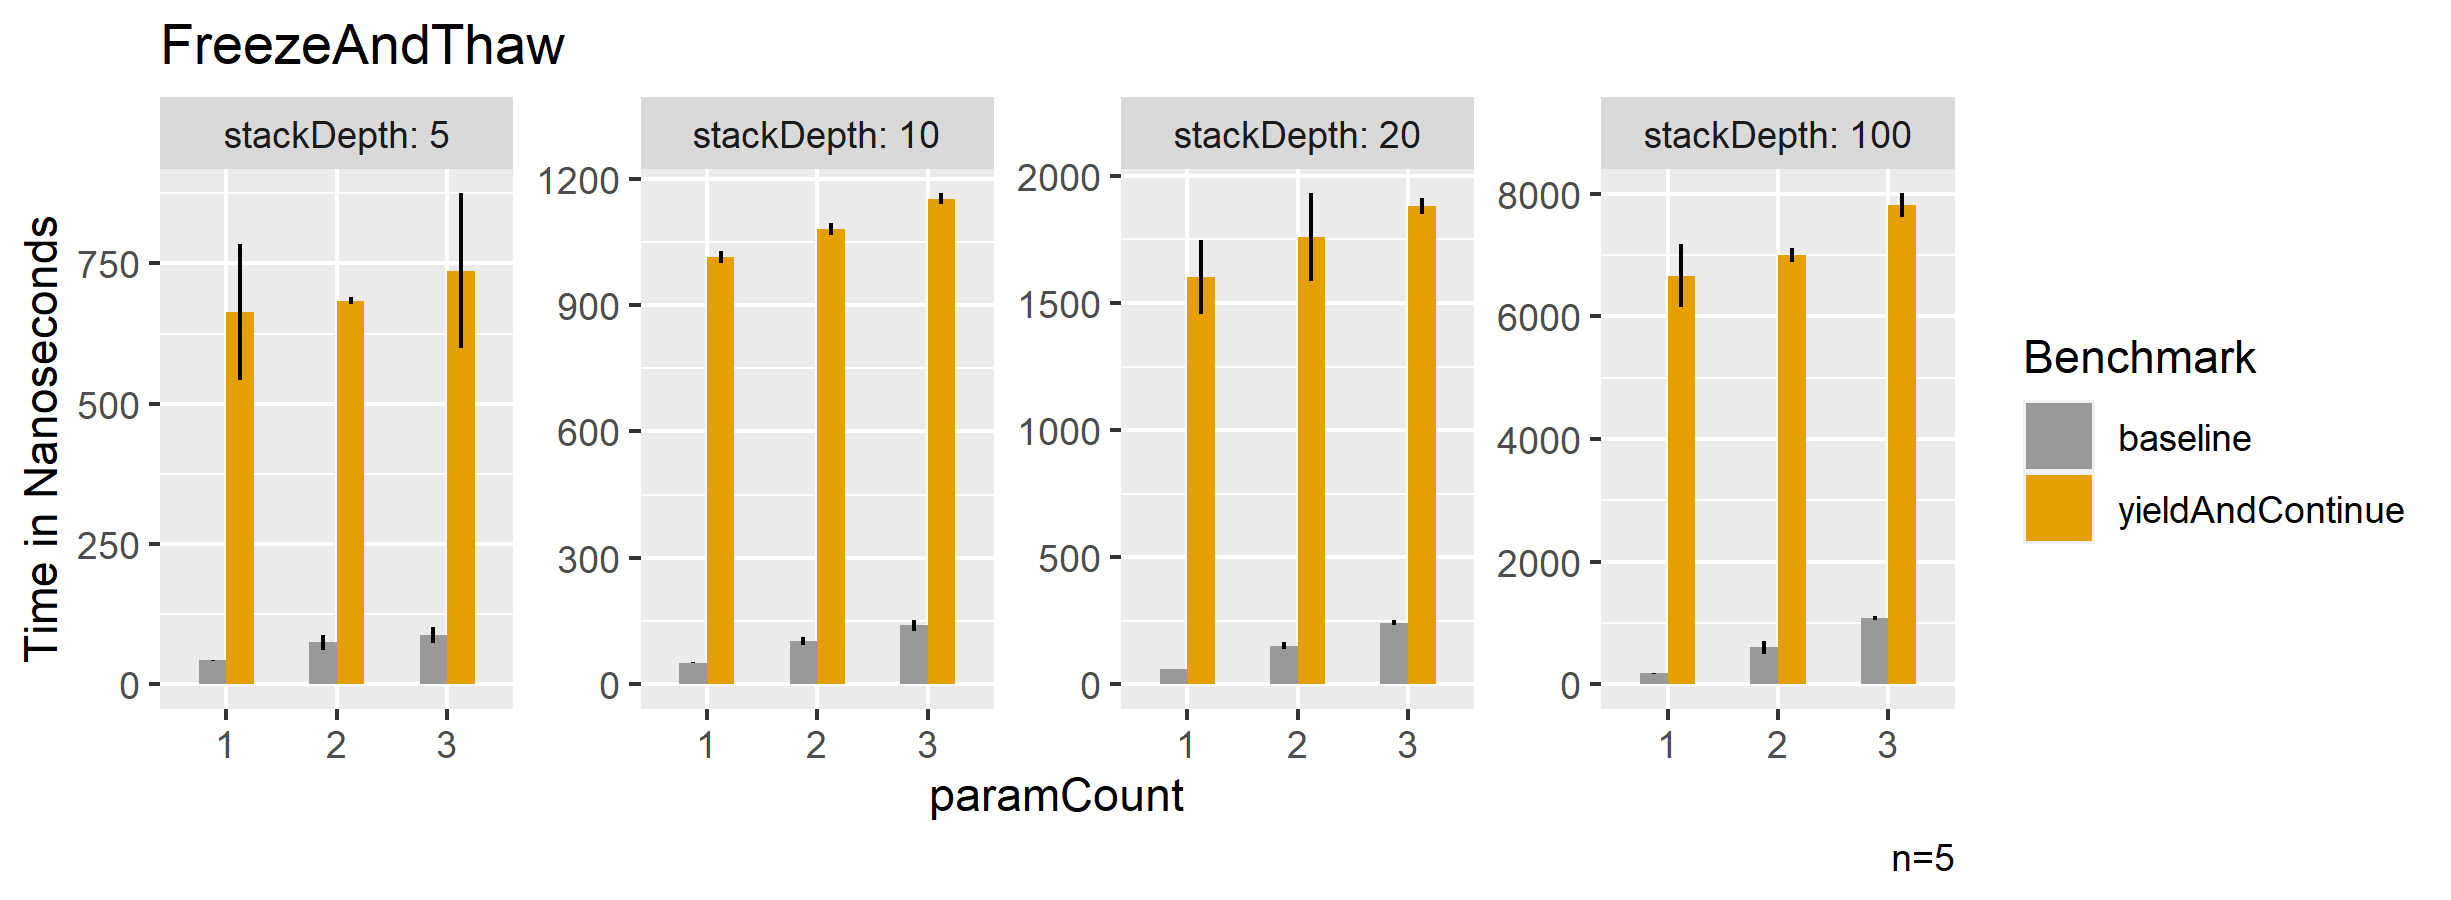
\includegraphics[width=1.0\linewidth]{img/jmh/FreezeAndThaw.png}
  \end{subfigure}
  \caption{FreezeAndThaw}
\end{figure}

\subsection{OneShot}
The OneShot class has many functions. The names of those functions very clearly describe, what they do. The functions become increasingly more demanding. The first function just runs the method without yielding. The last one yields before and after each call. 

\begin{figure}[H]
  \centering
  \begin{subfigure}[b]{1.0\textwidth}
    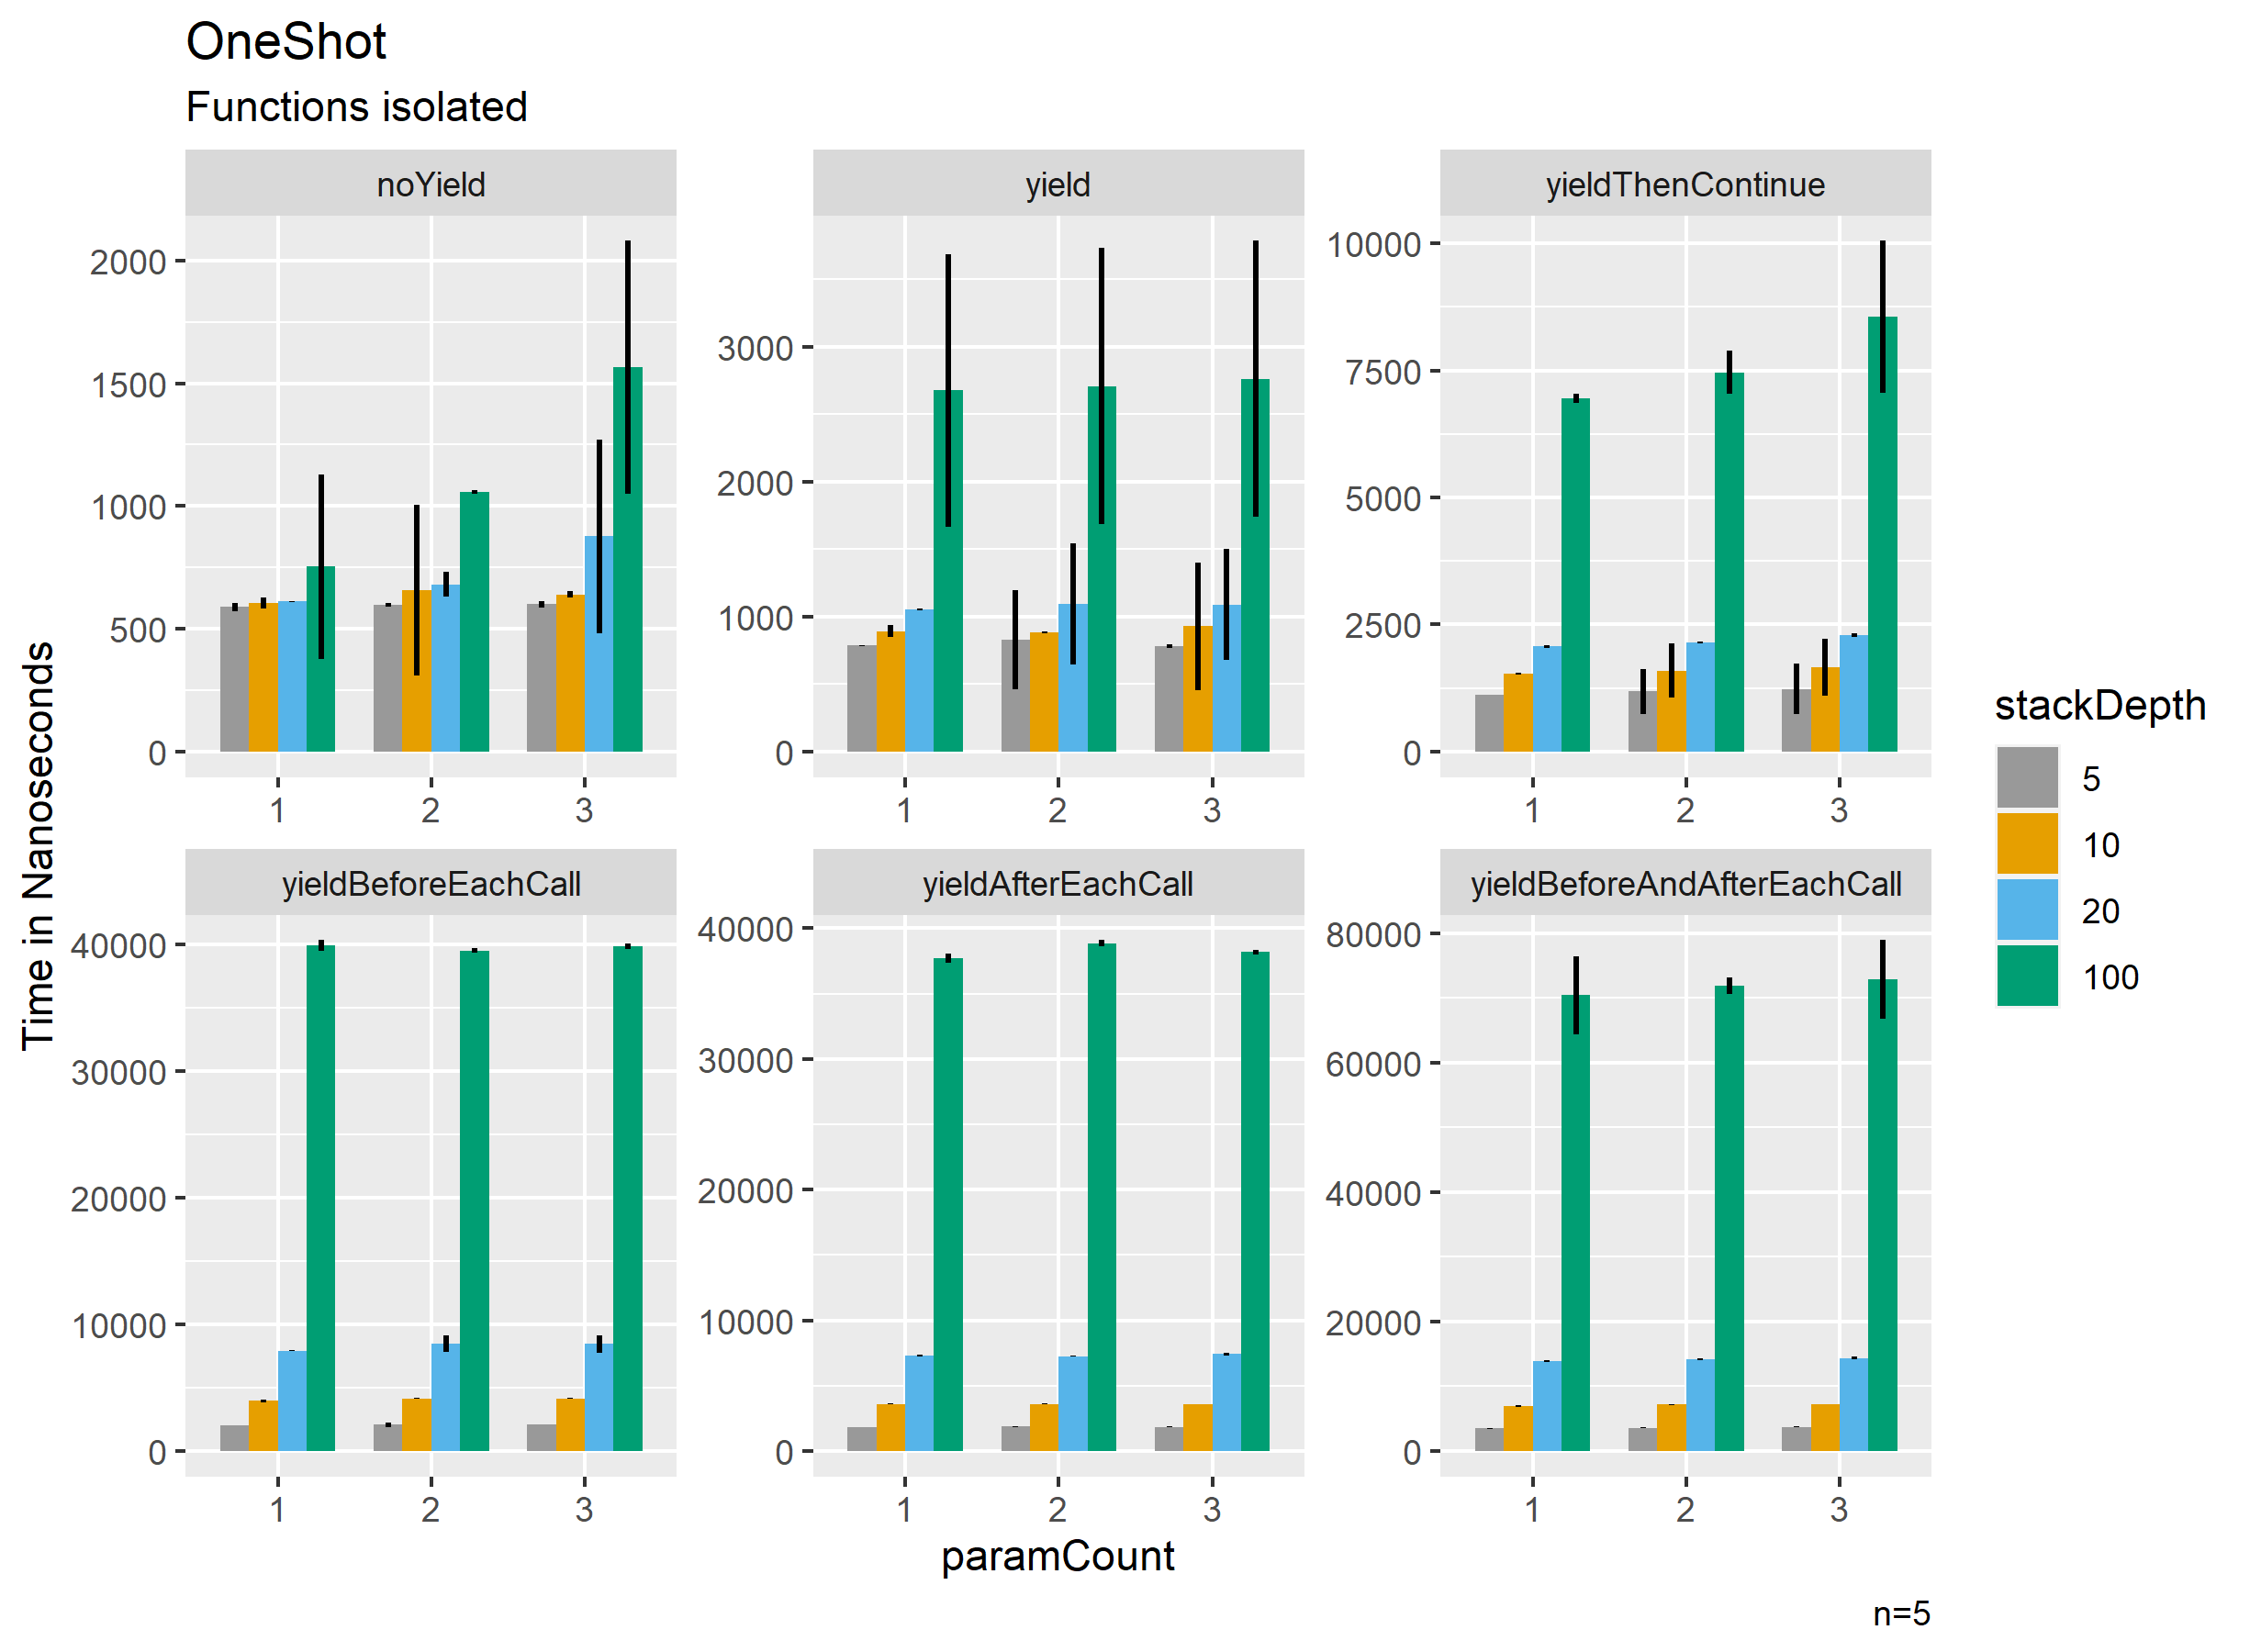
\includegraphics[width=1.0\linewidth]{img/jmh/OneShot.png}
  \end{subfigure}
  \caption{OneShot}
\end{figure}

One can also look at the individual functions in an isolated matter. One can immediately see that an increase in stack depth results in an increase in time. An increase in parameter count also seems to impact the time it takes to finish the task. One can observe it at a stack depth of 100.


\begin{figure}[H]
  \centering
  \begin{subfigure}[b]{1.0\textwidth}
    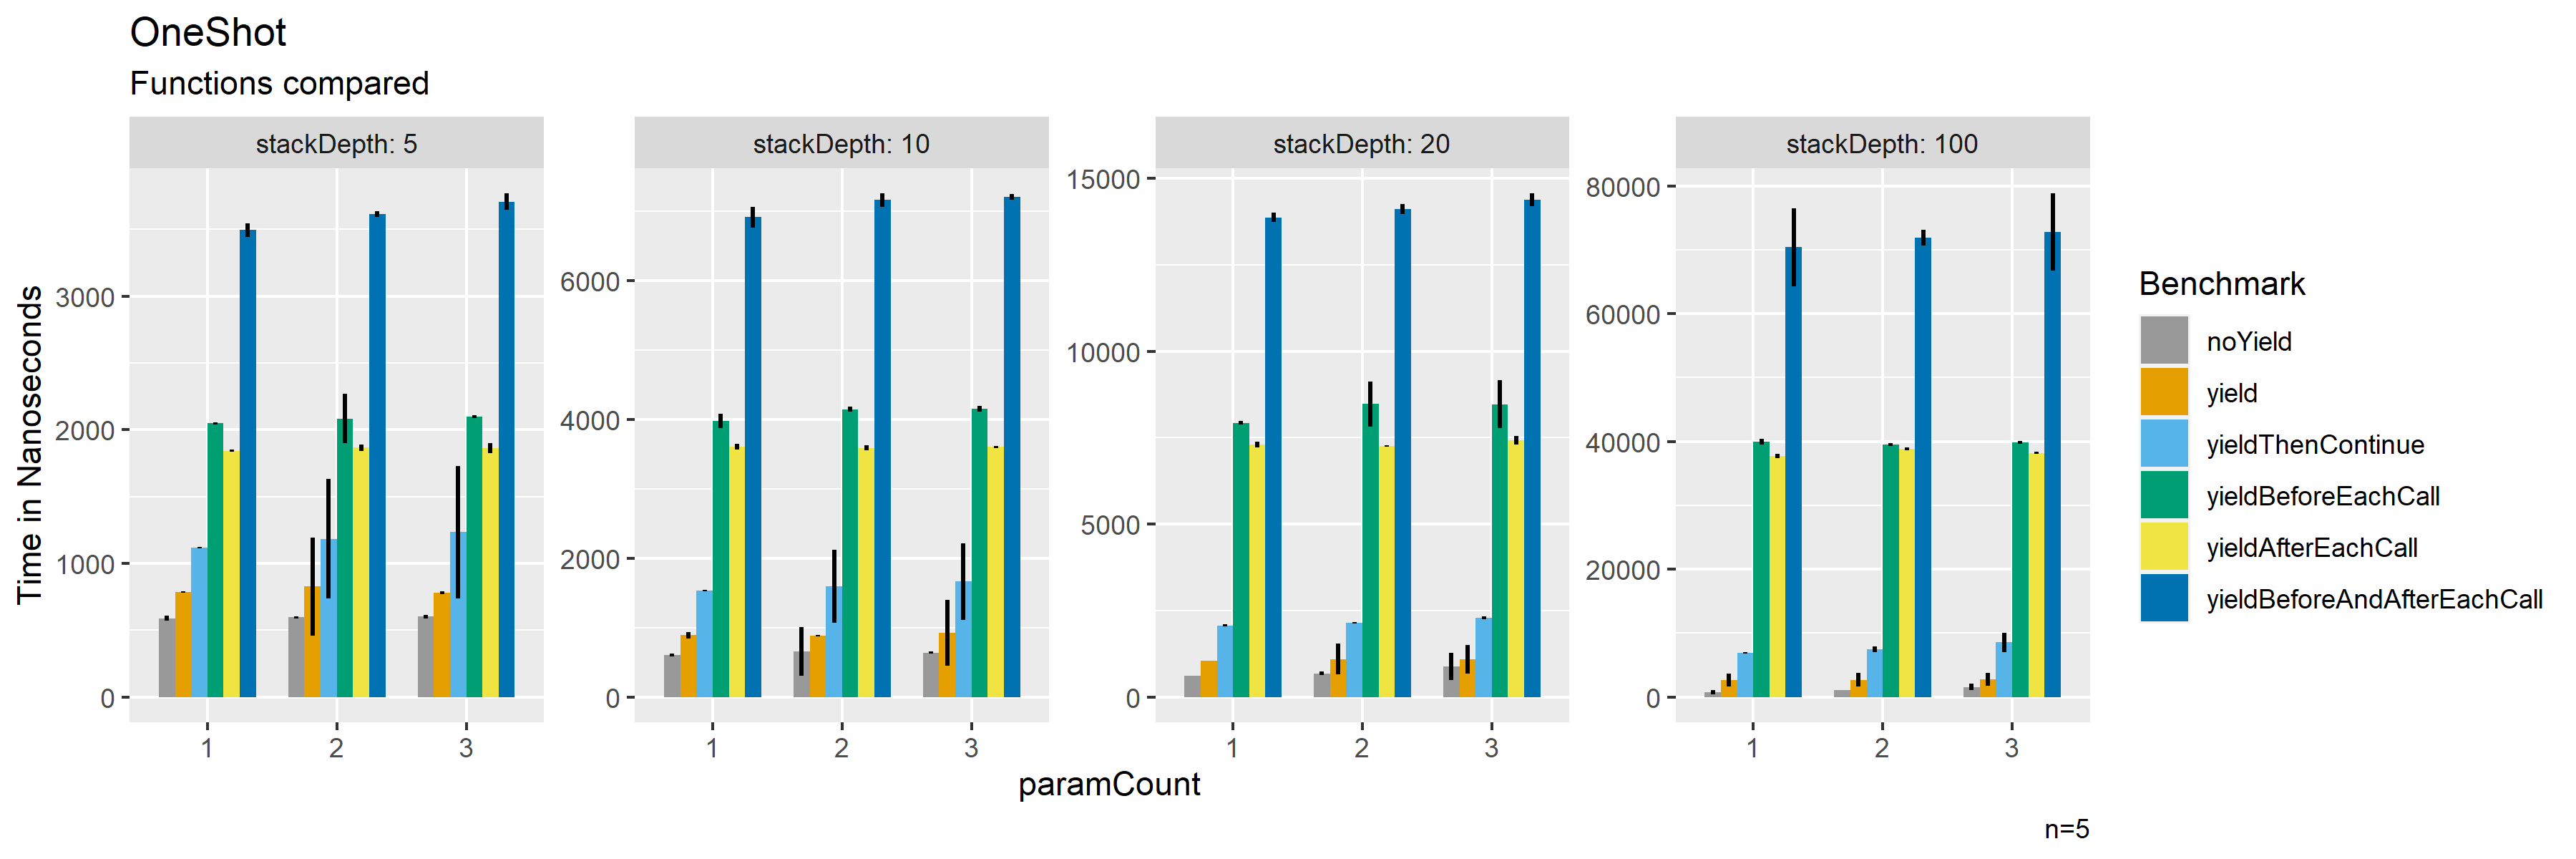
\includegraphics[width=1.0\linewidth]{img/jmh/OneShot2.png}
  \end{subfigure}
  \caption{OneShot}
\end{figure}





\subsection{Oscillation}
Here the continuation oscillates between a minimum and a maximum stack depth. It freezes at the maximum and continues afterwards.
One expectation here was that an increase in repetitions increases the time it takes to complete the task. This expectation has proven to be true. Another expectation was, that the bigger the difference from the minimal depth to the maximum depth is, the more time it would take to finish the task. This has also proven to be true.

\begin{figure}[H]
  \centering
  \begin{subfigure}[b]{1.0\textwidth}
    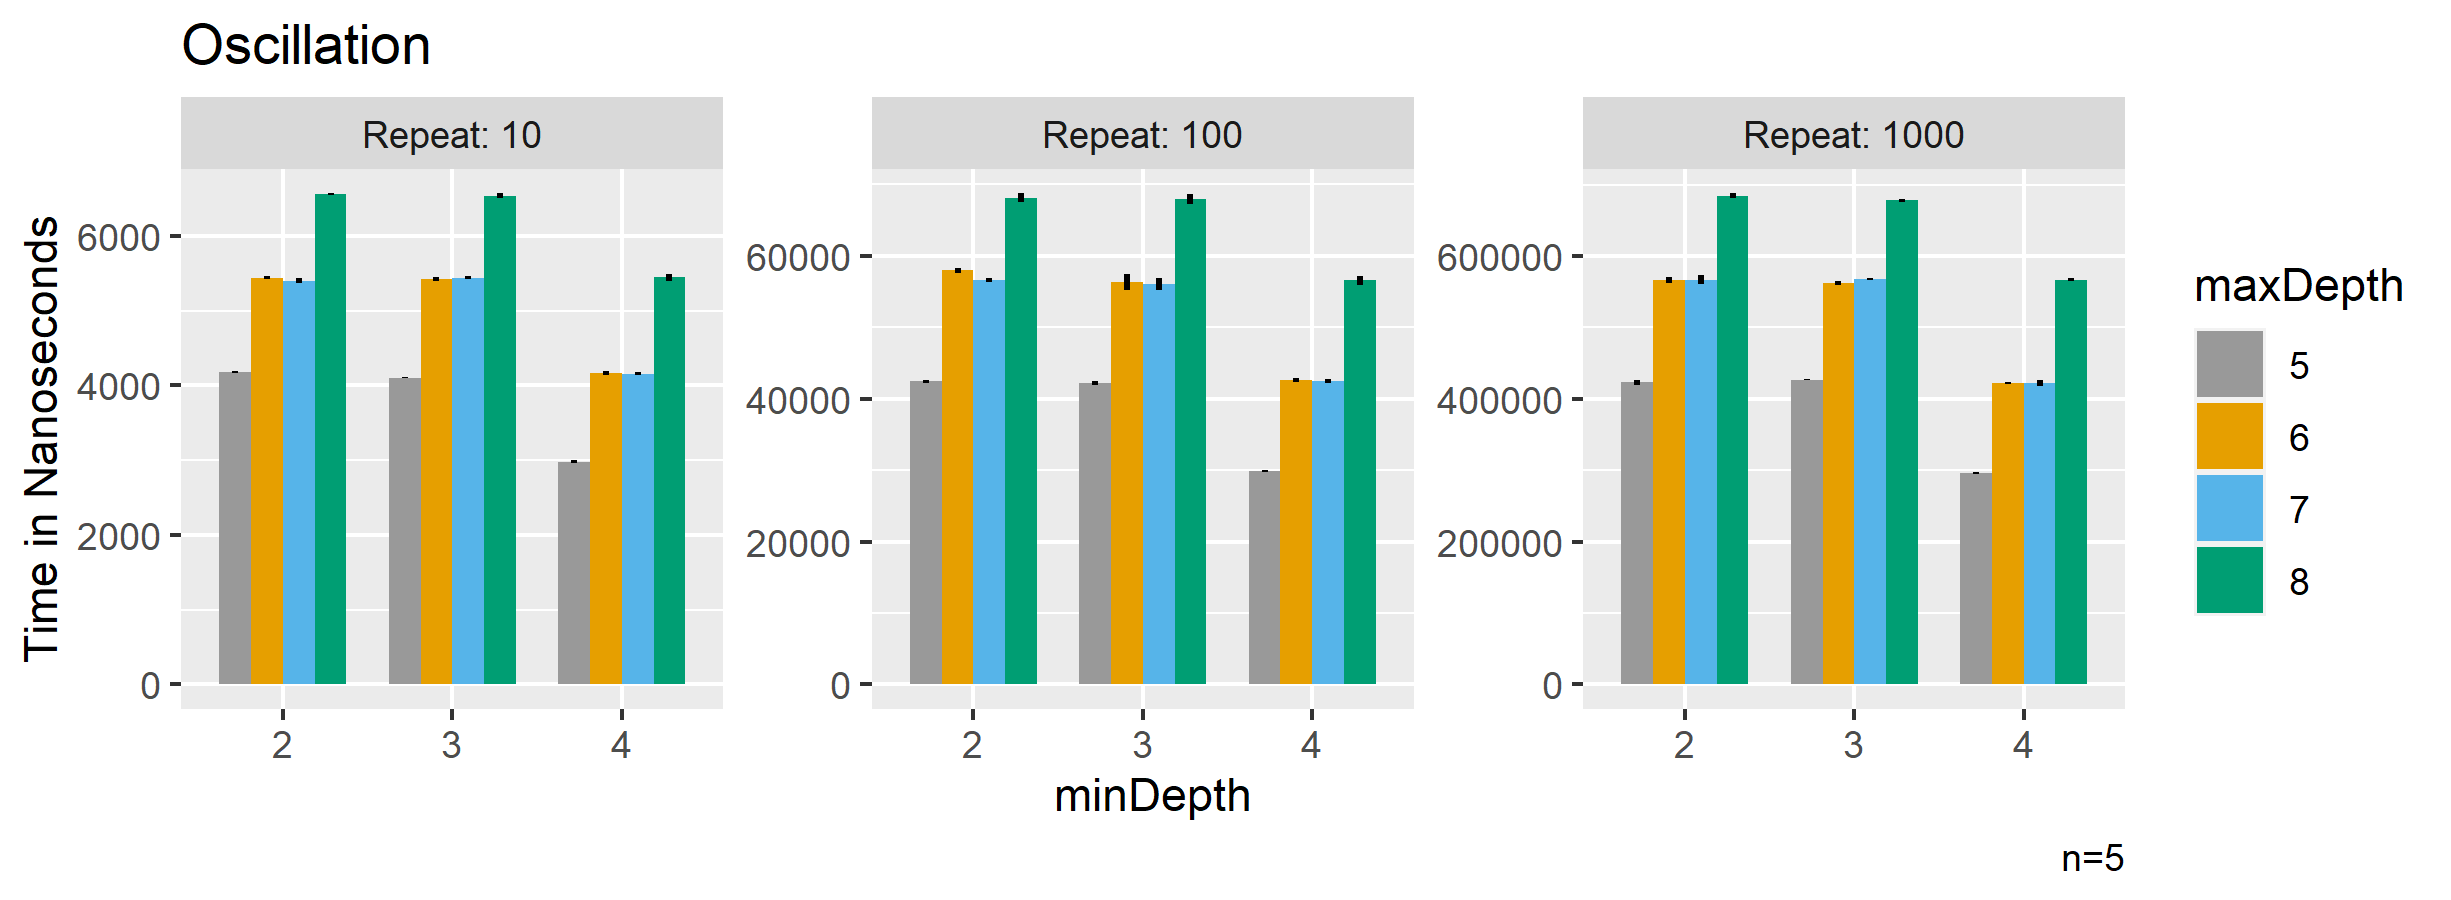
\includegraphics[width=1.0\linewidth]{img/jmh/Oscillation.png}
  \end{subfigure}
  \caption{Oscillation}
\end{figure}




\section{Footprint \& Performance}

\myparagraph{Experimental Setup}
Three Java classes are used in this experiment: EchoServerThread, EchoServerVThread, and Responder.
EchoServerThread and EchoServerVThread are almost identical. They both start a server that listens for requests on port 5566. Once a request is made, they start a separate thread, which runs the Responder class. Then they will continue to listen for further requests. The difference between the two classes is, that the EchoServerThread class utilizes kernel threads, while the EchoServerVThread class uses virtual threads. The Responder class sends a valid HTTP 1.1 header. Then it will echo the request it received.
\\
\\
Requests will be made using ApacheBench. All requests will be made with a concurrency of 100. Instead of running ApacheBench once with for example 1.000.000 requests, a shell script will be used. The shell script will then instead call ApacheBench 100 times in a row, with each run making 10.000 requests. This is done to remove ApacheBench as a potential bottleneck since it might not be fit to run 1.000.000 requests in a single process.
\\
\\
There will be two different kinds of measurement series:
\\
The first one is being recorded with VisualVM.
\\
The second one is recorded with JProfiler.
\\
There are multiple reasons for that. First off all a profiler might influence the measurements. Running similar tests with different profilers should improve the accuracy of the results. Also exporting the data is not possible using VisualVM. JProfiler allows one to export all measurements and model them as one wants to.

\myparagraph{Observed Values}
Heap size using VisualVM and JProfiler.
\\
Time to finish all requests using ApacheBench.


\subsection{Results - Profiler: VisualVM}
Virtual threads in orange and kernel threads in blue.
\\
\\
Looking at the scatter plots, one can immediately see that the virtual threads seem to not only perform better but also much more consistent than the kernel threads. When trying to model the results with linear regression, the first impression is further verified: The graph trying to model the virtual thread results is very precise. The margin for error is very small. On the other hand, the graph trying to model the kernel threads has a much bigger margin for error. This proves to be true in all 3 measurement series.

\begin{figure}[H]
  \centering
  \begin{subfigure}[b]{1.0\textwidth}
    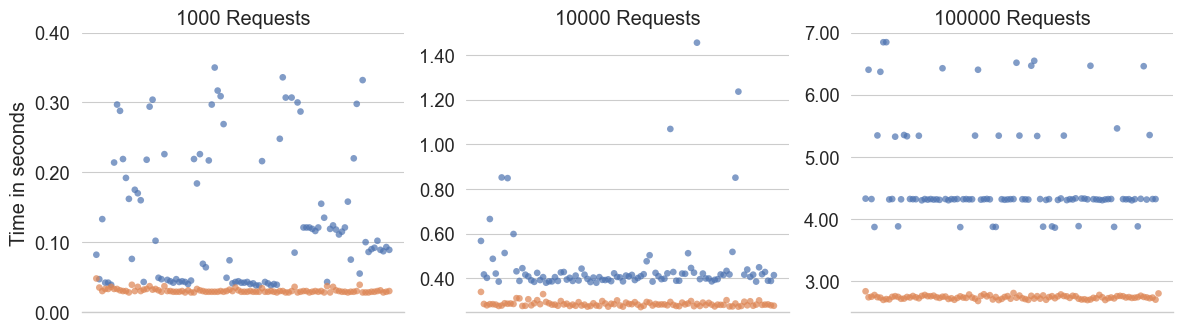
\includegraphics[width=1.0\linewidth]{img/footprint/scatter-100.png}
  \end{subfigure}
  \par\medskip % force a bit of vertical whitespace
  \begin{subfigure}[b]{1.0\textwidth}
    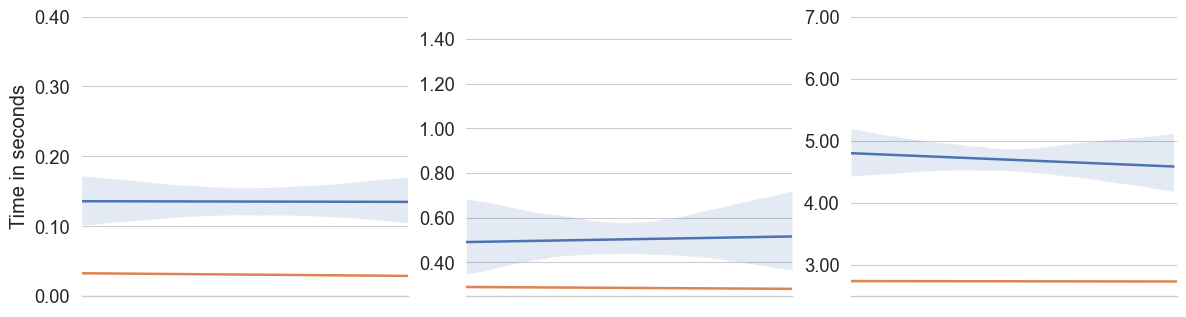
\includegraphics[width=1.0\linewidth]{img/footprint/linres-100.png}
  \end{subfigure}
  \caption{Time - Scatter \& Linear Regression - n=100 - VisualVM}
\end{figure}

Modeling the same results using boxplots allows one to take a closer look at the details. The 1000 requests series using virtual threads has a median of 30ms. The first and the third quartile are each 1ms above and below the median. Therefore 50\% of all the runs were completed between 29ms and 31ms. The 1000 requests series using kernel threads has a median around 100ms. The first quartile is slightly below 50ms and the third quartile is slightly above 200ms. That results in a spread of more than 150ms in the 50\% box.
\\
\\
The 10.000 requests series is more balanced: The 50\% box of the virtual threads series spans from 279ms to 289ms, resulting in a span of 10ms. The median is at 284ms. The 50\% box of the kernel threads series spans from 395ms to 430ms, resulting in a span of 35ms. The median is at 415ms. Any run that took longer than 480ms was considered an outlier for the kernel thread series and was not plotted. There are 10 such outliers.
\\
\\
In the 100.000 requests series, the 50\% box of the virtual threads run is slightly bigger than 25ms. The 50\% box of the kernel threads is slightly smaller than 20ms. Therefore this is the first series, in which the 50\% box spans a smaller range for the kernel threads. When one looks at the corresponding scatter plot, one can see, that there are more than 20 out of 100 runs, in which kernel threads needed more than 5 seconds to finish a run. Also, there are around 10 more runs, which were finished in less than 4 seconds. These 30 runs were considered outliers. No such outliers can be observed in the virtual thread series. Therefore, virtual threads perform more consistently once again.

\begin{figure}[H]
  \centering
  \begin{subfigure}[b]{1.0\textwidth}
    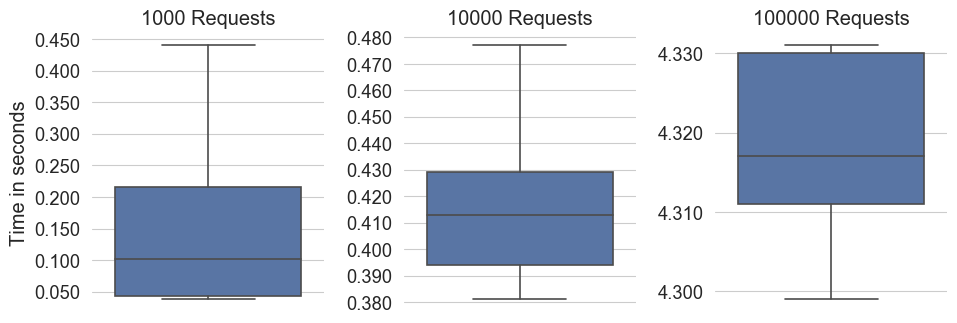
\includegraphics[width=1.0\linewidth]{img/footprint/boxplots-t-100.png}
  \end{subfigure}
  \par\medskip % force a bit of vertical whitespace
  \begin{subfigure}[b]{1.0\textwidth}
    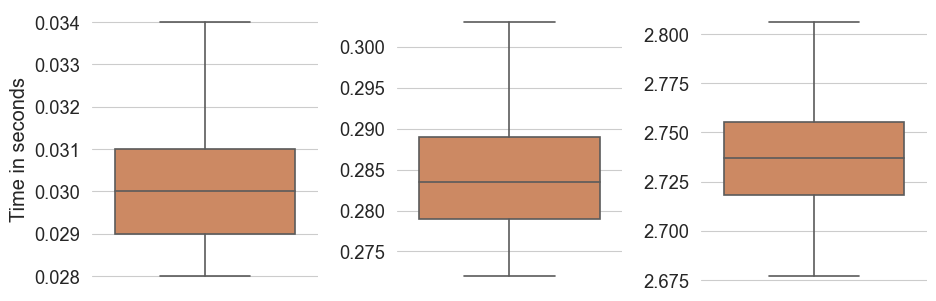
\includegraphics[width=1.0\linewidth]{img/footprint/boxplots-vt-100.png}
  \end{subfigure}
  \caption{Time - Boxplot - n=100 - VisualVM}
\end{figure}




\pagebreak
\subsection{Results - Profiler: JProfiler}
Virtual threads in orange and kernel threads in blue.
\\
\\
In the previous chapter the series with 1000 requests per run stuck out. Kernel threads performed especially more inconsistent in that series. Therefore the same experiment was run again here. Additionally, the number of runs was increased from 100 to 1000.

\begin{figure}[H]
  \centering
  \begin{subfigure}[b]{0.45\textwidth}
    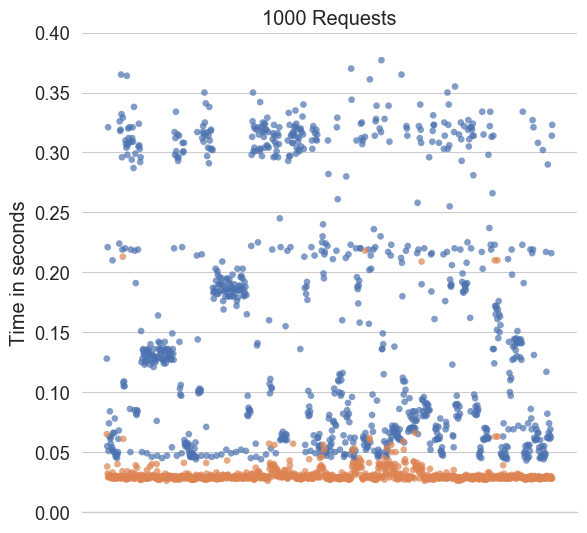
\includegraphics[width=1.0\linewidth]{img/footprint/scatter-1000.png}
  \end{subfigure}
  \begin{subfigure}[b]{0.45\textwidth}
    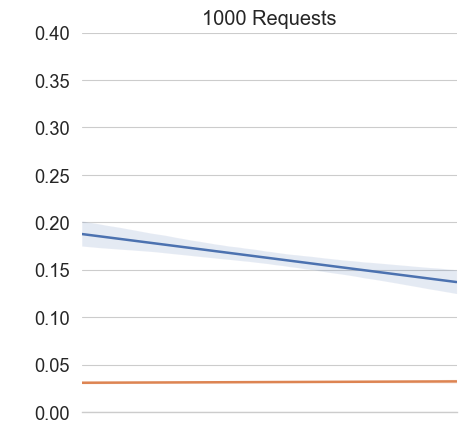
\includegraphics[width=1.0\linewidth]{img/footprint/linres-1000.png}
  \end{subfigure}
  \caption{Time - Scatter \& Linear Regression - n=1000 - JProfiler}
\end{figure}

Looking at the boxplots one can see, that the virtual threads performed similarly to before. The median is at 29ms, the 50\% box spans from 28ms to 30ms. The median of the kernel thread series is slightly higher than before. The 50\% box spans a range that is bigger than 100ms.

\begin{figure}[H]
  \centering
  \begin{subfigure}[b]{0.45\textwidth}
    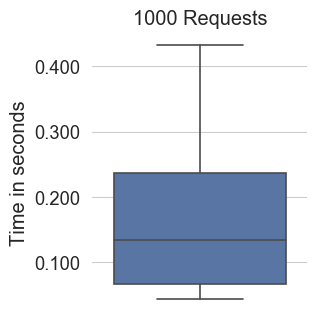
\includegraphics[width=1.0\linewidth]{img/footprint/boxplots-t-1000.png}
  \end{subfigure}
  \begin{subfigure}[b]{0.45\textwidth}
    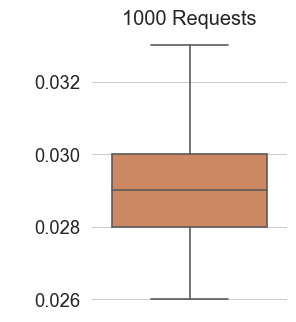
\includegraphics[width=1.0\linewidth]{img/footprint/boxplots-vt-1000.png}
  \end{subfigure}
  \caption{Time - Boxplot - n=1000 - JProfiler}
\end{figure}


Additionally, the heap usage is monitored this time around. Virtual threads use less heap space. They also are more consistent in their heap usage.


\begin{figure}[H]
  \centering
  \begin{subfigure}[b]{0.45\textwidth}
    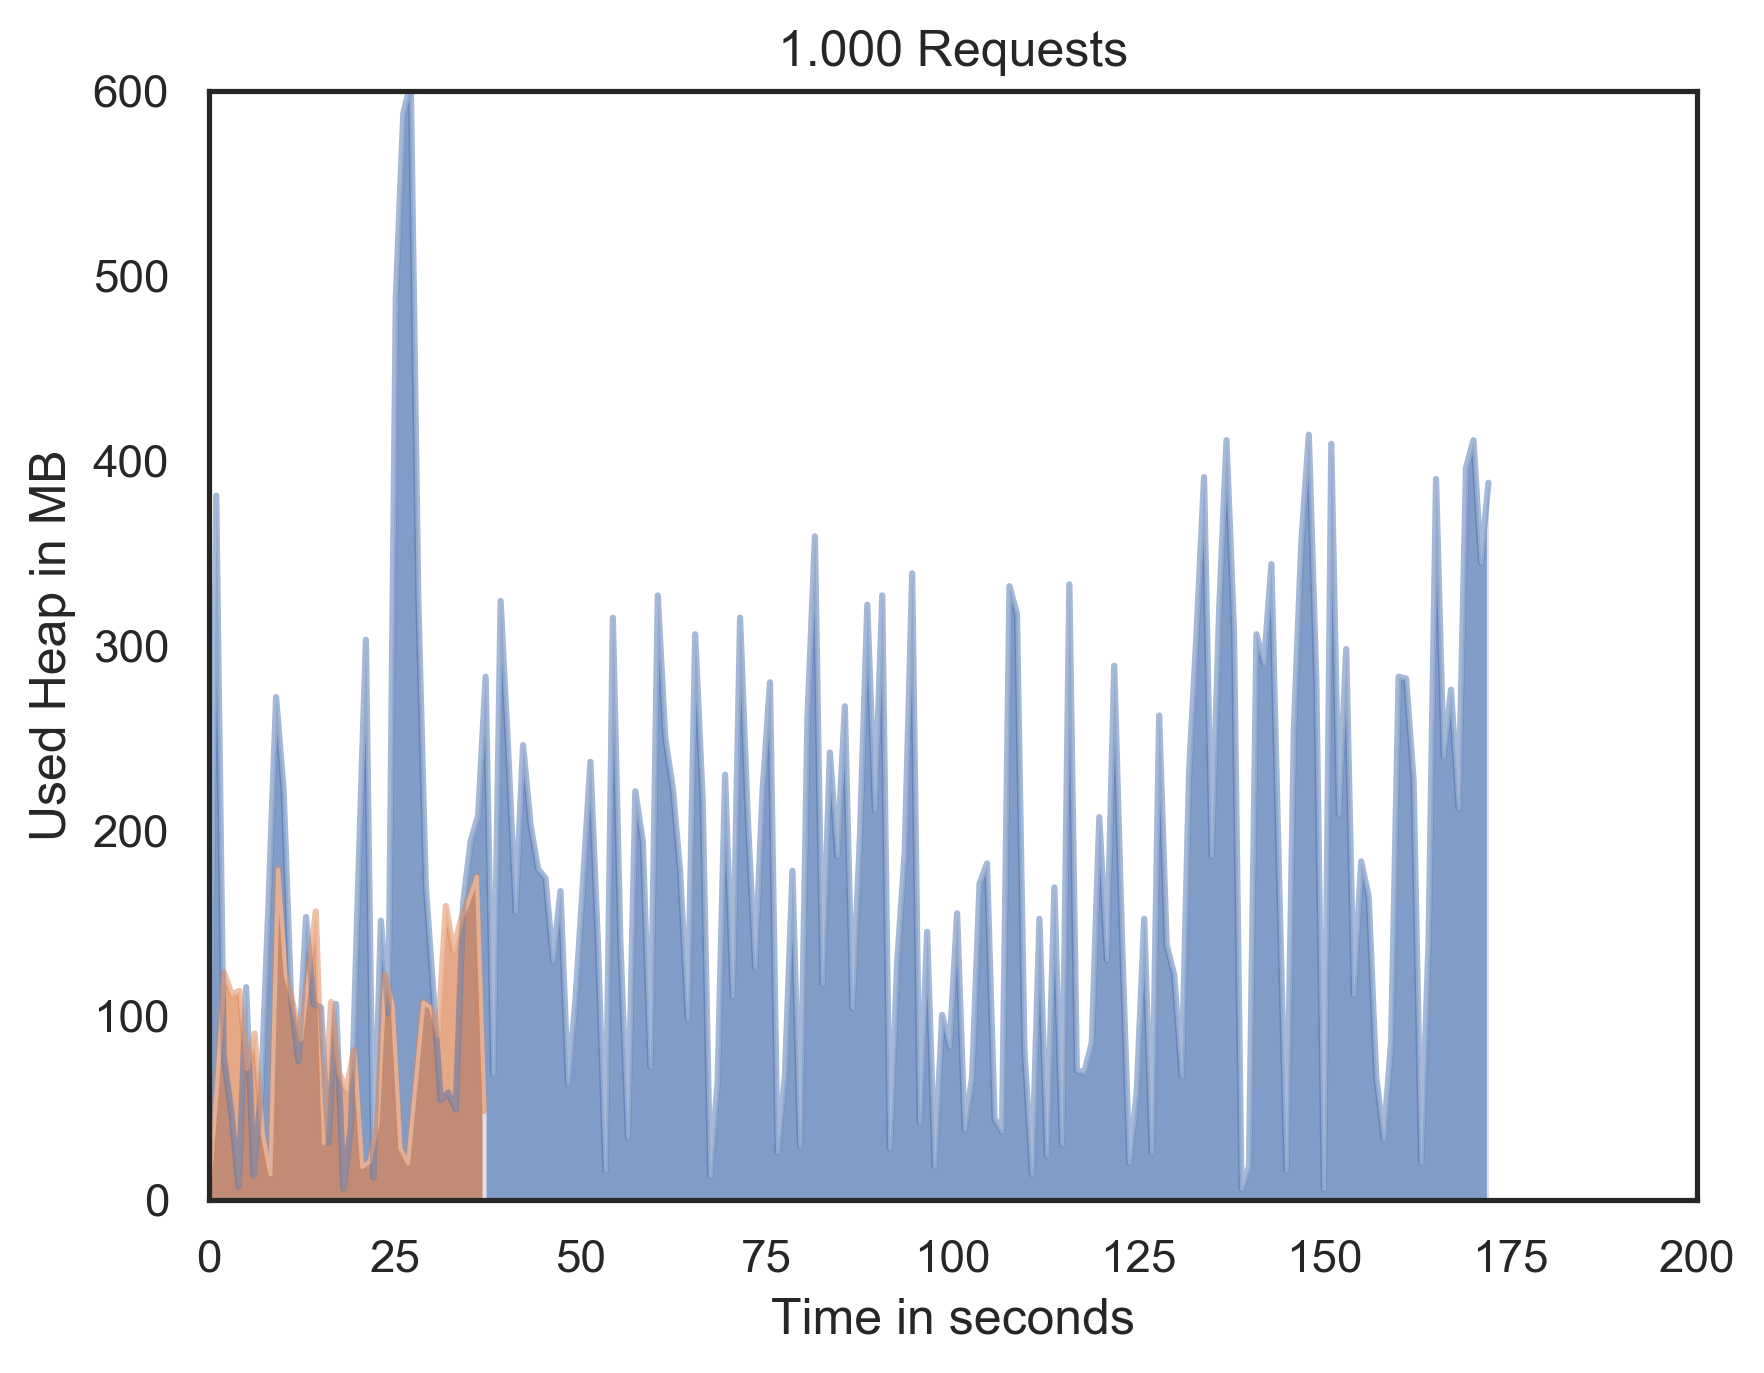
\includegraphics[width=1.0\linewidth]{img/footprint/heap_1000_line.png}
  \end{subfigure}
  \begin{subfigure}[b]{0.3\textwidth}
    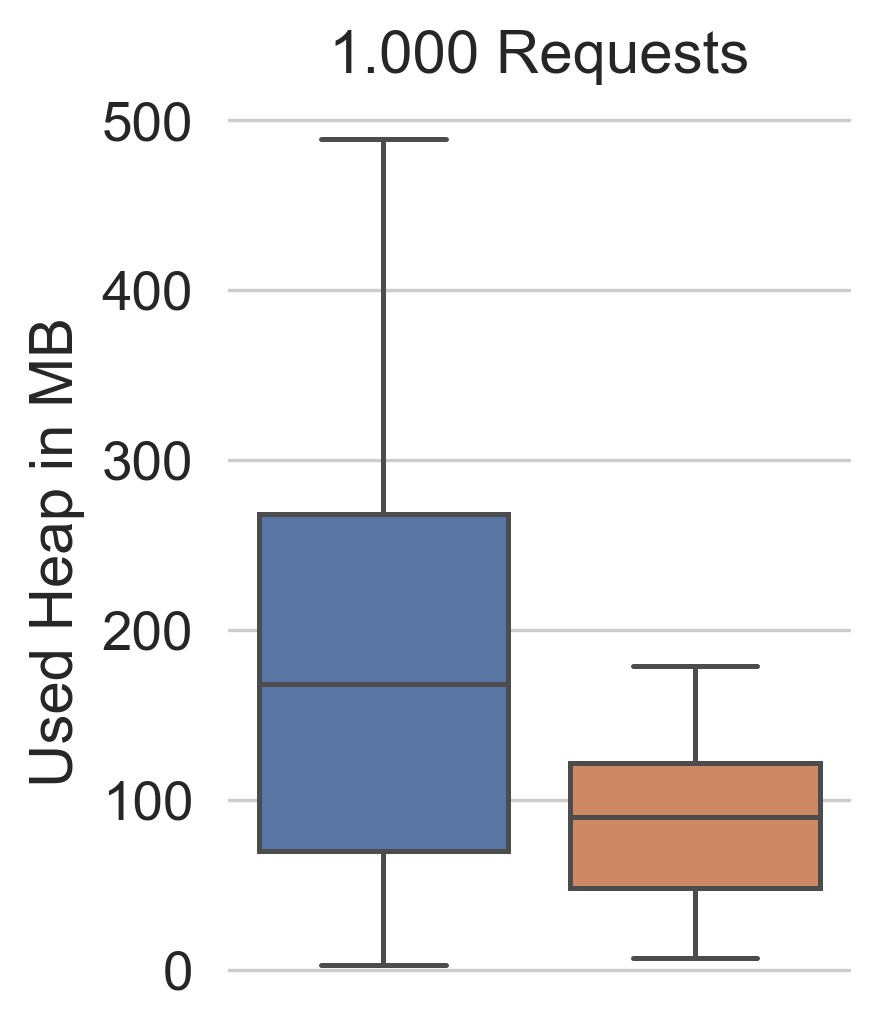
\includegraphics[width=1.0\linewidth]{img/footprint/heap_1000_box.png}
  \end{subfigure}
  \caption{Heap Usage - n=1000 - JProfiler}
\end{figure}

\pagebreak
The following series measures 10.000 requests, ran 500 times. Originally this series was intended to be ran 1000 times. That was not possible, because the Linux kernel consistently killed the EchoServerThread process at around 600 runs.
\\
\\
Virtual threads perform better and more consistent once again. Most runs were finished faster than 300ms. Looking at the kernel threads, the majority of runs were finished around 500ms. There also is a significant minority of runs finishing around 800-900ms.
\begin{figure}[H]
  \centering
  \begin{subfigure}[b]{0.45\textwidth}
    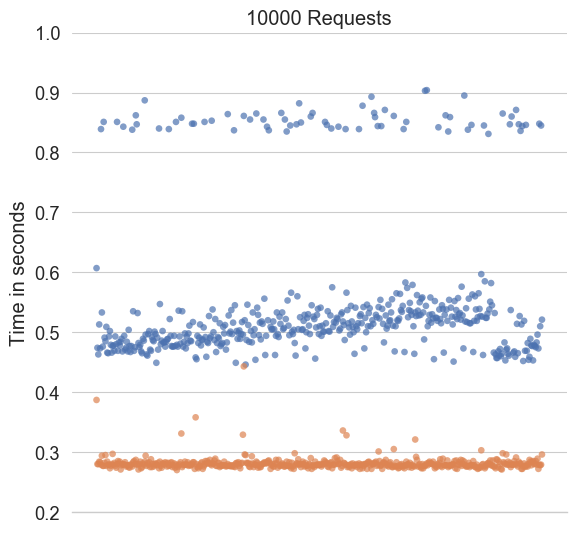
\includegraphics[width=1.0\linewidth]{img/footprint/scatter-500.png}
  \end{subfigure}
  \begin{subfigure}[b]{0.45\textwidth}
    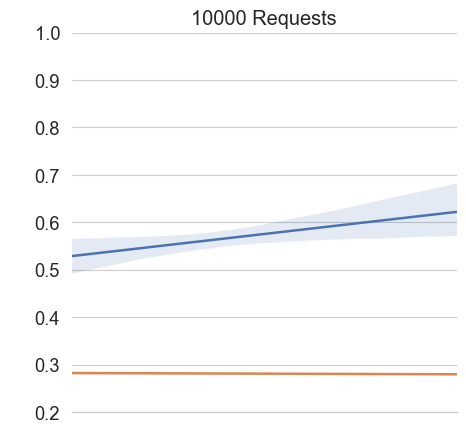
\includegraphics[width=1.0\linewidth]{img/footprint/linres-500.png}
  \end{subfigure}
  \caption{Time - Scatter \& Linear Regression - n=500- JProfiler}
\end{figure}

The median of the virtual thread series is 278ms. The median of the kernel thread series is 513ms. That is a decrease of more than 40\%. Also, the virtual thread 50\% box spans an area of 5ms here, while the kernel threads span an area of around 50ms.

\begin{figure}[H]
  \centering
  \begin{subfigure}[b]{0.45\textwidth}
    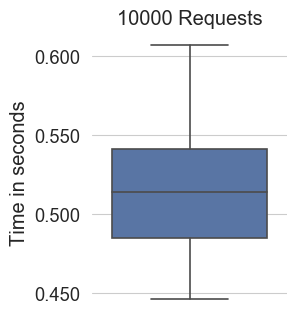
\includegraphics[width=1.0\linewidth]{img/footprint/boxplots-t-500.png}
  \end{subfigure}
  \begin{subfigure}[b]{0.45\textwidth}
    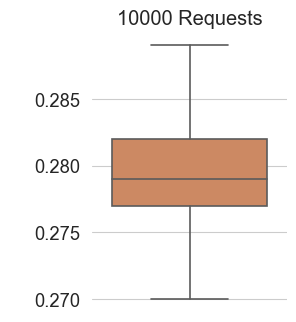
\includegraphics[width=1.0\linewidth]{img/footprint/boxplots-vt-500.png}
  \end{subfigure}
  \caption{Time - Boxplot - n=500 - JProfiler}
\end{figure}

Once again, the heap usage is significantly higher using kernel threads. The median of the kernel thread series is 200MB, while the virtual thread series has a median of 100MB. 

\begin{figure}[H]
  \centering
  \begin{subfigure}[b]{0.45\textwidth}
    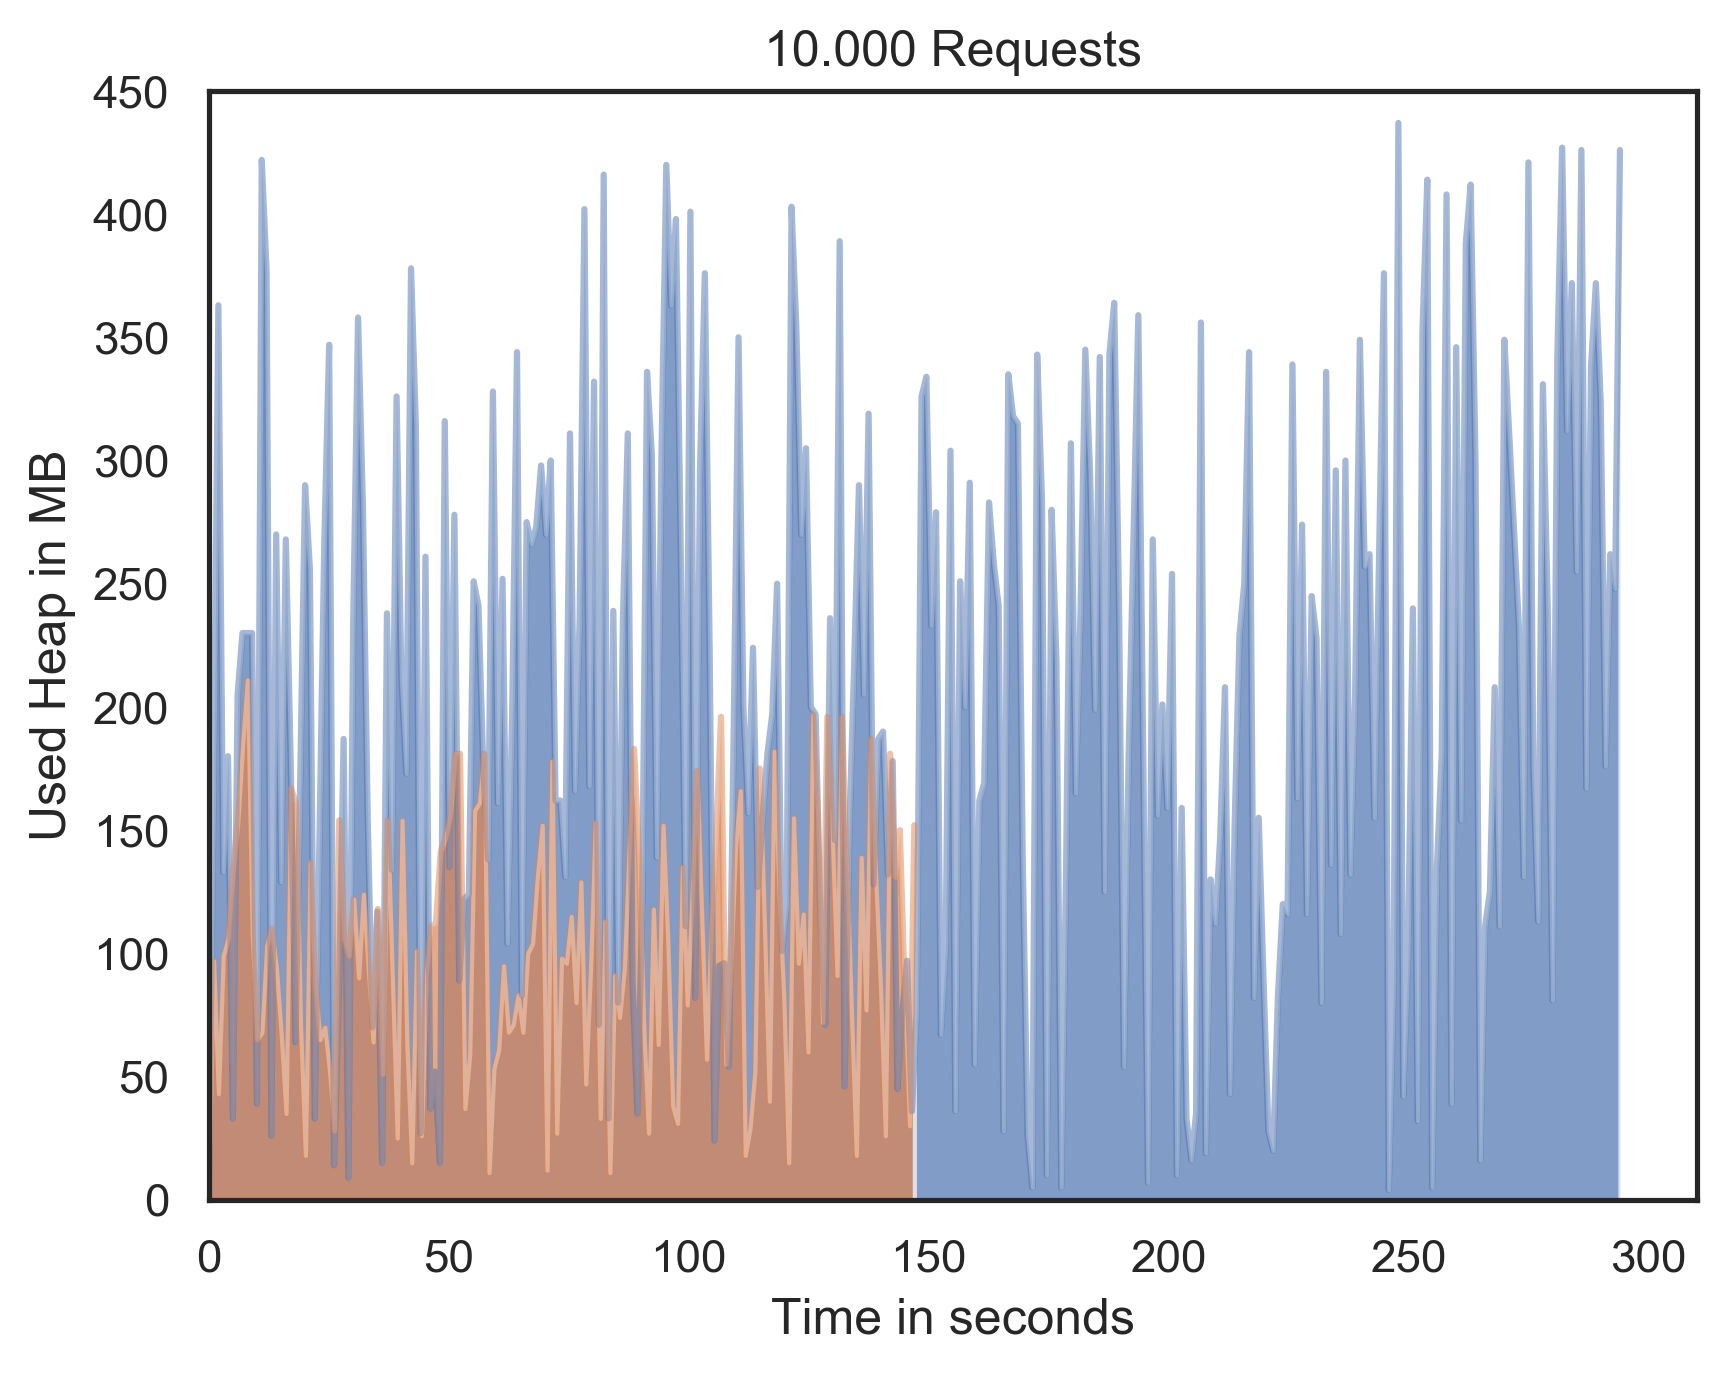
\includegraphics[width=1.0\linewidth]{img/footprint/heap_500_line.png}
  \end{subfigure}
  \begin{subfigure}[b]{0.3\textwidth}
    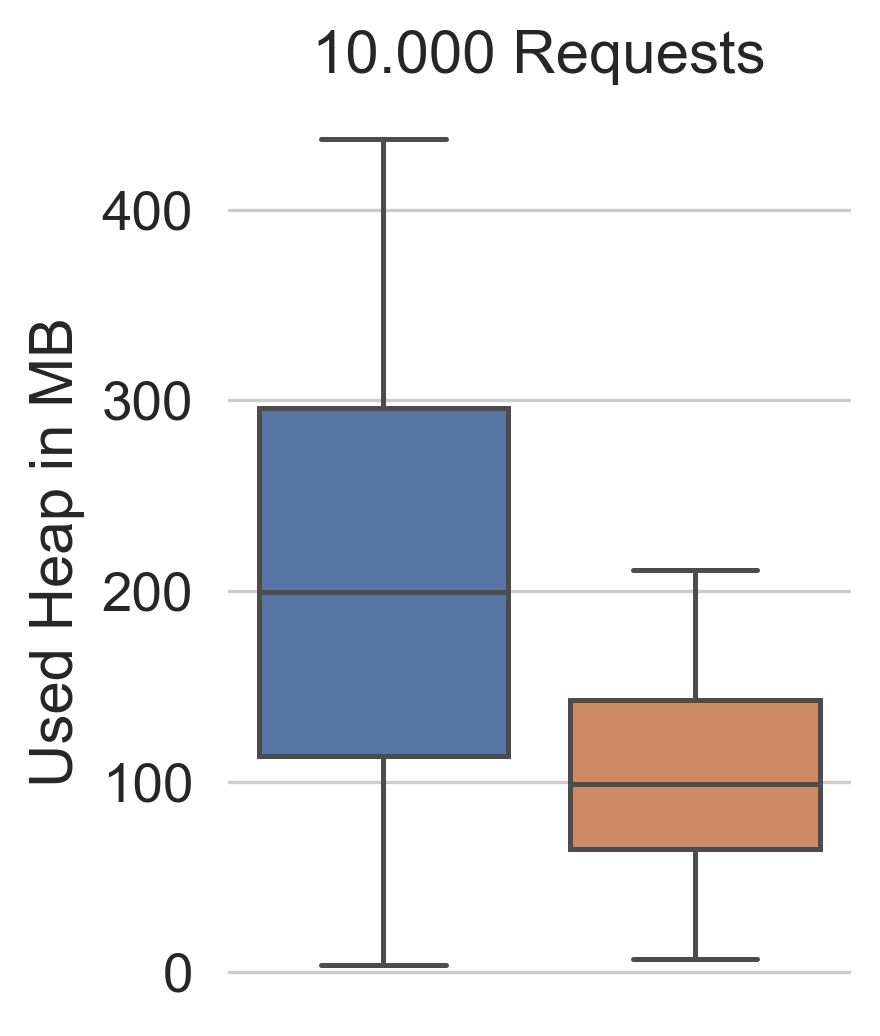
\includegraphics[width=1.0\linewidth]{img/footprint/heap_500_box.png}
  \end{subfigure}
  \caption{Heap Usage - n=500 - JProfiler}
\end{figure}




\section{Evaluation of the implementation Loom}

Wrapping up the observations from the experiments:
\begin{itemize}
  \item Virtual threads are faster.
  \item Virtual threads perform more consistently.
  \item Virtual threads require less heap space for the same task.
\end{itemize}

The transition from kernel to virtual threads is, or at least envisioned to be, effortless. A free 33\% increase in performance and a 50\% decrease in footprint is not only something existing pieces of software written in Java will appreciate but also a strong argument for newer projects to use Java. Therefore, it is very much in Oracle's interest, that the project will successfully be finished as soon as possible. 
\\
\\
Also, project Loom is already part of the newer OpenJDK releases. Old APIs, that were not compatible with virtual threads, are already being reworked. As an example, the network API has already been changed and supports virtual threads now.
\\
\\
With all these observations in mind, it is highly unlikely, that the project won't be finished. It will provide a significant performance increase to the Java ecosystem.